\chapter{Проектирование микросервисной архитектуры с помощью UML диаграмм. }
\textbf{Аннотация.} \textit{Приведено подробное описание спроектированной микросервисной архитектуры с использованием UML диаграмм, демонстрирующих как физическое, так и логическое распределение компонентов. Отражено разделение системы на микросервисы с акцентом на их взаимное взаимодействие через стандартизированные интерфейсы. Приведено описание внешних интерфейсов, обеспечивающих связь с внешними клиентами и другими системами. Отражена модель внутренних интерфейсов, определяющих обмен данными между микросервисами. Приведены UML диаграммы развертывания, иллюстрирующие физическую инфраструктуру, включая использование sidecar-компонентов. Приведены диаграммы последовательности, отражающие все стадии прохождения запросом пути от клиента до сервера и обратно.}

В данной главе представлено подробное описание спроектированной микросервисной архитектуры, отражающее как физическое распределение компонентов, так и их логическую взаимосвязь. Используя UML диаграммы развертывания, продемонстрировано разделение системы на микросервисы с акцентом на стандартизированные интерфейсы для обмена данными между ними, а также описаны внешние интерфейсы, обеспечивающие связь с клиентами и другими системами.

Также приведены диаграммы последовательности, иллюстрирующие все стадии маршрутизации запросов от клиента до сервера и обратно. Такой комплексный подход, включающий использование sidecar-компонентов для управления трафиком и интеграцию систем мониторинга, позволяет получить достоверную модель архитектуры, готовую к реализации и дальнейшему тестированию.


\section{Описание архитектуры системы с помощью диаграммы развертывания.}
\textbf{Аннотация.} \textit{Отражены ключевые аспекты взаимодействия компонентов на основе стандартной UML-нотации. Приведено подробное описание архитектуры системы с разделением на физические и виртуальные узлы. Разработана методика группировки контейнеров в поды для отображения ролей приложений и их sidecar-компонентов. Отражено распределение программных артефактов по физическим серверам и виртуальным машинам в рамках кластера k3s. Приведены зависимости между компонентами, иллюстрирующие потоки данных и сетевые связи. Разработаны схемы, демонстрирующие интеграцию системного мониторинга с помощью fluentbit и Jaeger.Отражены принципы управления трафиком через Istio sidecar для обеспечения безопасности и надежности. Приведено использование Helm-чарта как средства автоматизированного развертывания сервисов. }

На диаграмме развертывания (см. рис. \ref{pic:deployment-diagram-Istio}) система представлена с использованием Istio sidecar в каждом поде: Python-server, прокси‐сервер дополнены sidecar контейнерами, обеспечивающими перехват и маршрутизацию трафика. Такое решение упрощает контроль сетевых потоков и повышает наблюдаемость благодаря прямой интеграции с fluentbit, который собирает логи и метрики. Вариант без Istio (см. рис. \ref{pic:deployment-diagram-NOIstio}) показывает, как сервисы могут взаимодействовать напрямую, сохраняя более простую структуру развертывания, но при этом теряя автоматизированные возможности балансировки и политики безопасности. На обоих вариантах диаграммы отражено, что каждая виртуальная машина в кластере k3s содержит отдельные поды: один с основным приложением и sidecar (или без него), и дополнительный pod с fluentbit. Helm-чарт используется для автоматизации развертывания, что позволяет централизованно управлять конфигурациями. 

\begin{figure}[t]
    \centering
    \rotatebox{-90}{%
      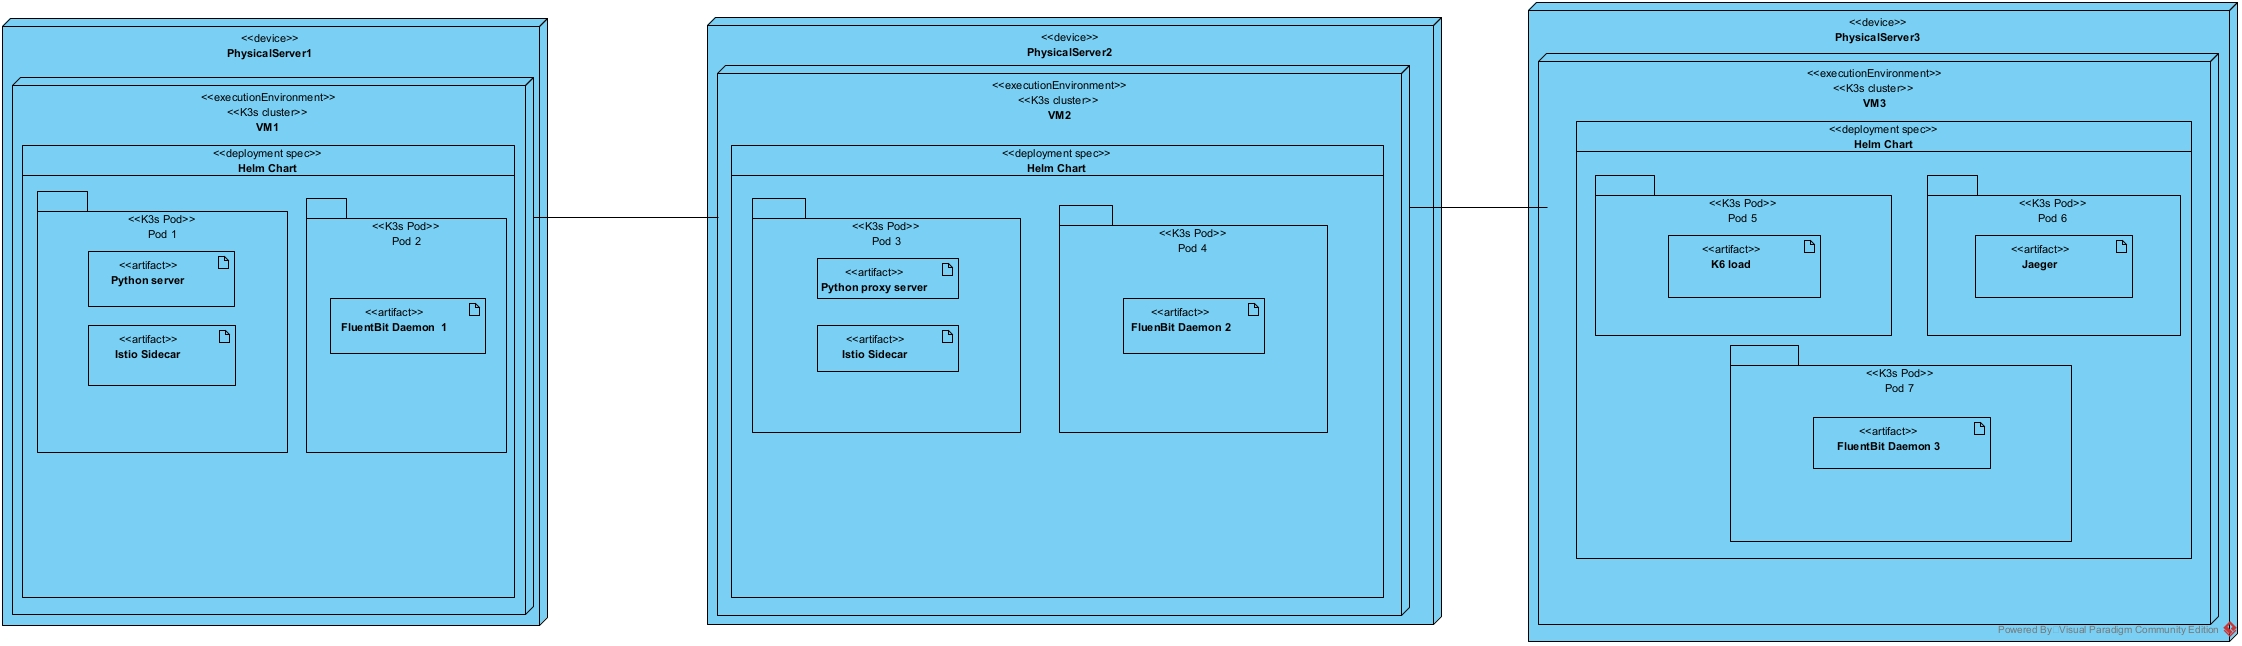
\includegraphics[width=\textheight, keepaspectratio]{./img/DeploymentIstio.jpg}%
    }
    \caption{Диаграмма развертывания версии с Isito}
    \label{pic:deployment-diagram-Istio}
  \end{figure}
  

  \begin{figure}[t]
      \centering
      \rotatebox{-90}{%
        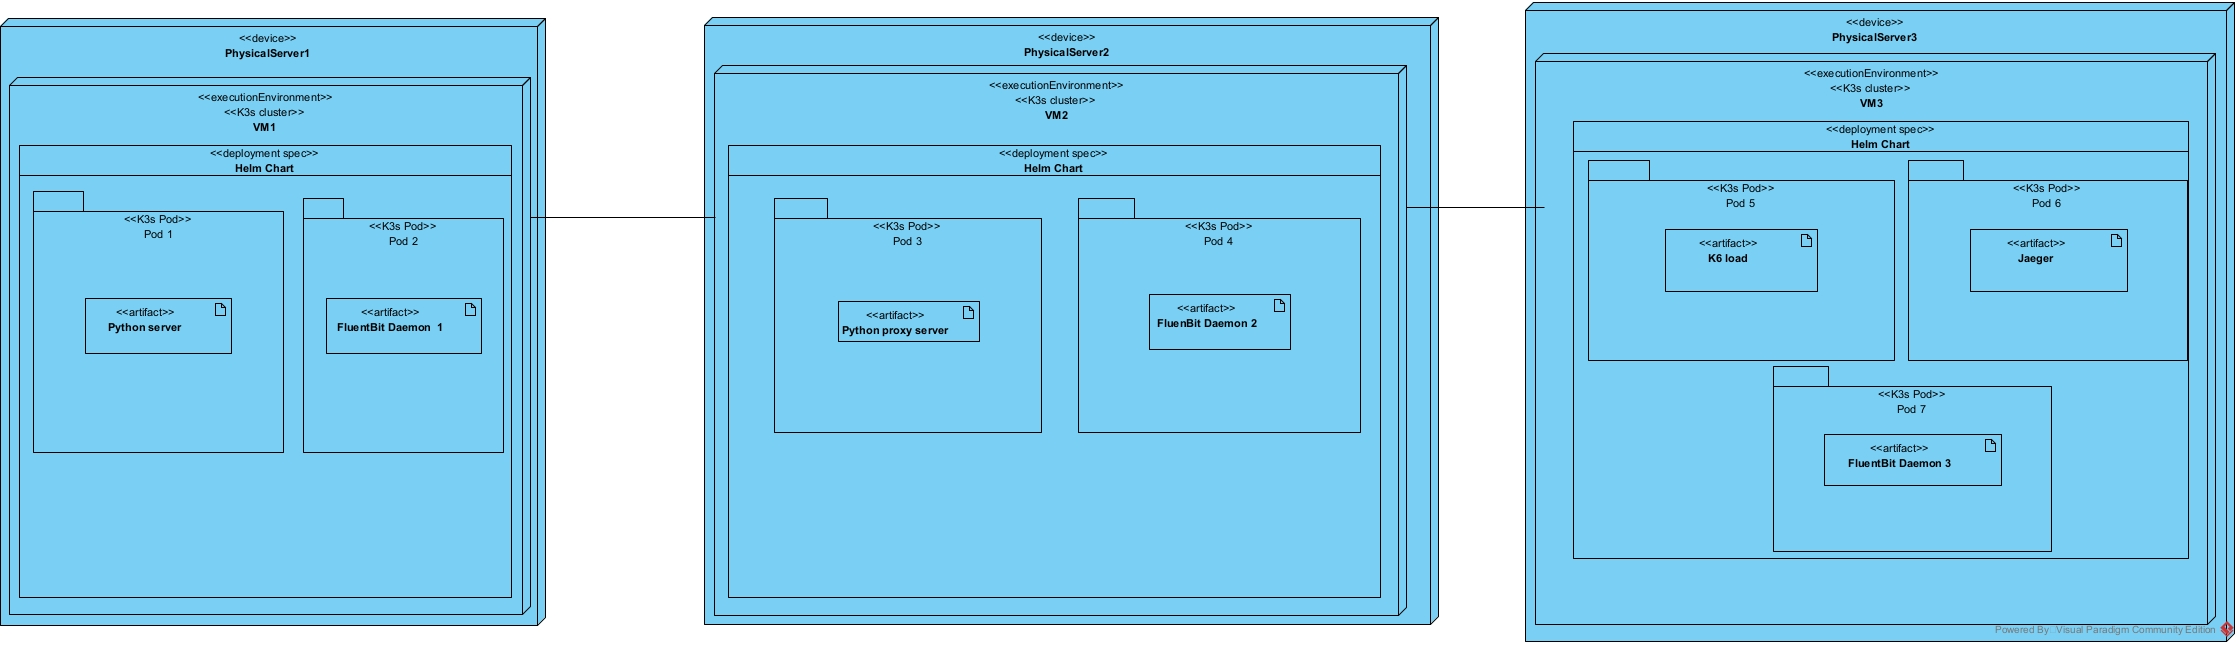
\includegraphics[width=\textheight, keepaspectratio]{./img/DeploymentNOIstio.jpg}%
      }
      \caption{Диаграмма развертывания версии без Isito}
      \label{pic:deployment-diagram-NOIstio}
    \end{figure}



\section{Описание архитектуры системы с помощью диаграммы последовательности.}

\textbf{Аннотация.} \textit{Разработана модель коммуникаций, иллюстрирующая маршрутизацию запросов от инициирующего сервиса к конечному получателю. Приведено подробное описание последовательности обмена сообщениями между сервисами, демонстрирующее логику взаимодействия. Отражено, как в версии с использованием Istio трафик проходит через sidecar-компоненты, обеспечивая дополнительный контроль и безопасность. Приведено сравнение с самописной реализацией, где обмен сообщениями осуществляется напрямую без промежуточного proxy-слоя. Разработана последовательность вызовов, охватывающая все ключевые этапы обработки запросов в системе. Отражены различия в производительности и надежности между обеими реализациями коммуникации сервисов.}

Диаграмма последовательности, представленная на (см. рис. \ref{pic:sequence-diagram-Istio}), демонстрирует прохождение трафика через Istio sidecar: клиент формирует запрос, прокси перенаправляет его в Istio, который дополнительно проверяет доступность основного сервиса и контролирует возможные сбои. Это даёт дополнительный уровень управления и безопасности, но требует промежуточной обработки.

Вариант без service mesh (см. рис. \ref{pic:sequence-diagram-NOIstio}) показывает более прямую схему обмена сообщениями: прокси общается с сервером напрямую, без дополнительного слоя Istio. Такая реализация может быть проще в настройке, но лишена встроенных возможностей мониторинга и контроля, которые предоставляет Istio.
 


\begin{figure}[t]
    \centering
    \rotatebox{-90}{%
      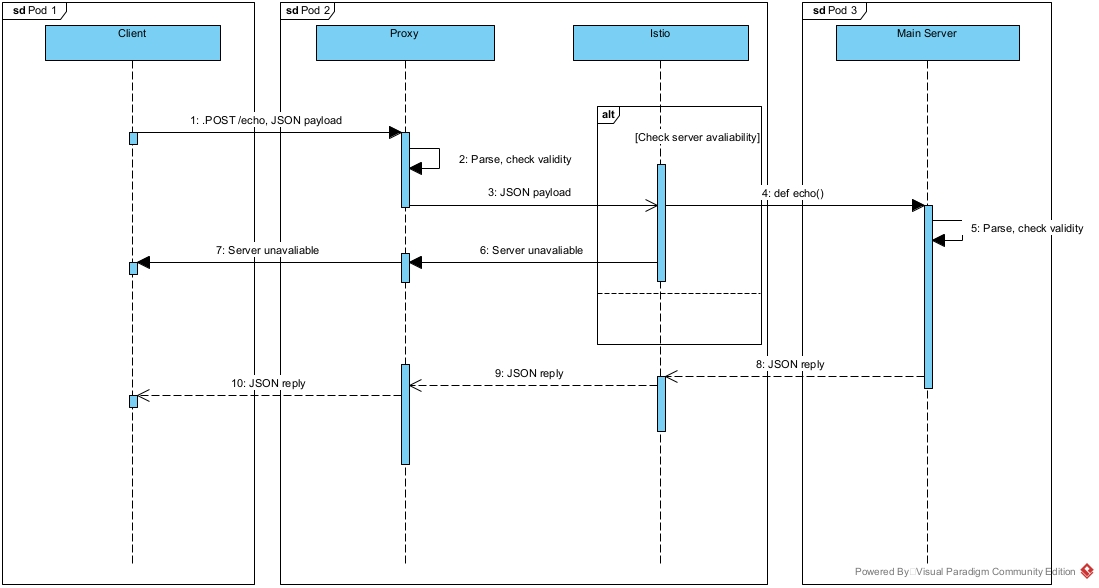
\includegraphics[width=\textheight, keepaspectratio]{./img/SequenceIstio.jpg}%
    }
    \caption{Диаграмма последовательности версии с Istio}
    \label{pic:sequence-diagram-Istio}
  \end{figure}


\begin{figure}[t]
      \centering
      \rotatebox{-90}{%
        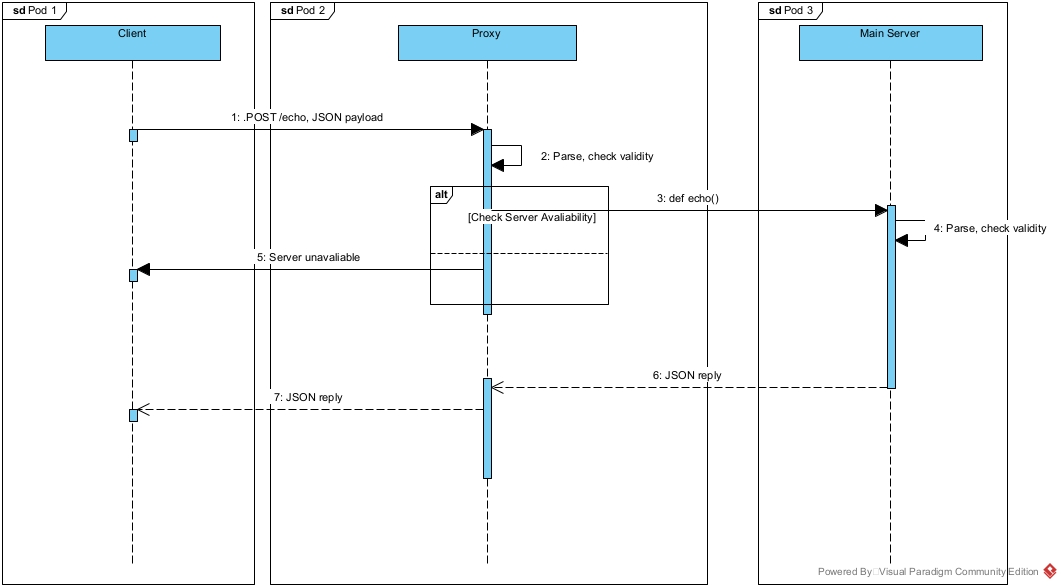
\includegraphics[width=\textheight, keepaspectratio]{./img/SequenceNOIstio.jpg}%
      }
      \caption{Диаграмма последовательности версии без Istio}
      \label{pic:sequence-diagram-NOIstio}
    \end{figure}
  


% Команда \texorpdfstring необходима, чтобы программа просмотра PDF документов
% верно отображала текст формул в панели оглавления.
% При отсутствии команды \texorpdfstring там, где она необходима, LaTeX выводит
% предупреждение "Token not allowed in a PDF string"


\section{Выводы}

\textbf{Аннотация.} \textit{Получена достоверная модель системы, полностью отражающая архитектуру, которая остается лишь реализовать. Спроектированы основные программные модули, включая сервер, прокси-сервер и модуль генерации нагрузки k6. Учтены особенности физической инфраструктуры с разделением на физические серверы и виртуальные машины в кластере k3s. Отражена интеграция data collector для сбора и централизованной передачи логов и трейсов. Приведена схема автоматизированного развертывания с использованием Helm-чарта для управления микросервисами. Итоговый результат – надежная и полная инженерная модель, готовая к непосредственной реализации и проведению тестов.}

В итоге проведённого проектирования и анализа можно заключить, что созданная модель микросервисной архитектуры учитывает все ключевые аспекты: от физической инфраструктуры и виртуальных машин в кластере k3s до логики взаимодействия сервисов в вариантах с Istio sidecar и без него. Подробно отражены потоки данных, маршрутизация и методы автоматизации развертывания, что формирует целостное представление о системе.

Разработанные диаграммы развертывания и последовательности подтвердили, что заложенные решения по управлению трафиком и сбору метрик (fluentbit, Jaeger) легко масштабируются и обеспечивают высокий уровень наблюдаемости. Таким образом, полученная модель является надёжной основой для дальнейшей реализации и проведения полноценных нагрузочных тестов.

%%% Local Variables:
%%% TeX-engine: xetex
%%% eval: (setq-local TeX-master (concat "../" (seq-find (-cut string-match ".*-3-pz\.tex$" <>) (directory-files ".."))))
%%% End:
